\documentclass[a4paper,12pt]{article}
\usepackage[utf8x]{inputenc}
\usepackage[T1]{fontenc}
\usepackage{lmodern}
\usepackage{a4wide}
\usepackage{textcomp}
\usepackage[english, czech]{babel}
\usepackage[pdftex, final]{graphicx}

\usepackage{hyperref}
%\usepackage{url}

%opening
\title{Zásuvný modul QGIS pro práci s~katastrálními daty}
\author{Anna Kratochvílová, Václav Petráš}

\newcommand{\klicslova}[2]{\noindent\textbf{#1: }#2}
\newcommand{\radekZkr}[2]{\textbf{#1} & #2 \\}
\setlength{\parskip}{1ex plus 1ex minus 1ex}
\begin{document}

\pagestyle{empty}
{
\newcommand{\napisCVUT}{ČVUT~v~Praze}
\newcommand{\napisFS}{Fakulta stavební}
\newcommand{\napisSVOC}{Studentská vědecká a odborná činnost}
\newcommand{\napisAK}{Akademický rok  2011/2012}
\newcommand{\napisObor}{Geoinformatika}
\newcommand{\napisKatedra}{Katedra mapování a kartografie}
\newcommand{\napisVedouci}{Ing. Martin Landa}
\newcommand{\napisAutor}{Anna Kratochvílová, Václav Petráš}
\newcommand{\napisRocnik}{1. magisterského}
\newcommand{\napisNazevI}{Zásuvný modul QGIS}
\newcommand{\napisNazevII}{pro práci s katastrálními daty}
% \newcommand{\napisNazevIII}{v systému GRASS}


%\colorbox{YellowOrange}{
\begin{minipage}{0.2\textwidth}

\includegraphics[width=3.7cm]{logo_cvut_modre}
\end{minipage}
%}
\hfill
%\colorbox{YellowOrange}{
\begin{minipage}{0.7\textwidth}
\begin{flushright}
\textsf{
\textbf{
\Large
\napisCVUT\\
\napisFS\\
\napisKatedra\\
}
\Large
\napisSVOC\\
\napisAK
}
\end{flushright}
\end{minipage}
%}


\begin{center}
\vfill
\textsf{
\textbf{
\Huge
\napisNazevI\\
\napisNazevII\\
% \napisNazevIII\\
}}
\vfill
\end{center}

\newcommand{\rtu}[2]{\textsf{#1}&\textsf{#2}\\}
\begin{tabular}{ll}
\rtu{Jméno a příjmení studenta:}{\napisAutor}
\rtu{Ročník, obor:}{\napisRocnik, \napisObor}
\rtu{Vedoucí práce:}{\napisVedouci}
% \rtu{Ústav:}{\napisKatedra}
\end{tabular}
}

\newpage
\pagestyle{empty}
\begin{abstract}
Cílem tohoto projektu je vytvoření zásuvného modulu (pluginu) pro program Quantum GIS,
který bude umožňovat práci s~daty (českého) katastru nemovitostí.
QGIS je rychle se rozvíjející  multiplatformní geografický informační systémem pod licencí GNU GPL.
Jeho grafické uživatelské rozhraní je napsáno v~jazyce C++ pomocí knihovny Qt. Plugin je napsán také v~jazyce C++.
Nový plugin pracuje s~daty katastru nemovitostí a to v~takzvaném novém výměnném formátu katastru označovaném VFK či NVF.
K~datům přistupuje pomocí ovladače knihovny OGR. Plugin by měl usnadnit vyhledávání a zobrazování
informací při práci s~daty katastru nemovitostí.
Zobrazení informací se uskutečňuje podobně jako u~webových aplikací, ovládání je tedy pro uživatele přívětivé a známé.
Plugin samozřejmě podporuje interakci s~mapou za použití funkcí QGISu.
Součástí pluginu je i možnost exportu listu vlastnictví a dalších výpisů.

\bigskip

\klicslova{Klíčová slova}{QGIS, OGR, VFK, NVF, katastr, ČÚZK, C++, zásuvný modul}
\end{abstract}

\selectlanguage{english}

\begin{abstract}
The goal of this project is to develop Quantum GIS plugin for Czech cadastral data.
QGIS is a rapidly developing cross-platform desktop Geographic Information System (GIS) released under the GNU GPL.
QGIS is written in C++, and uses the Qt library.
The plugin is developed in C++, too.
The new plugin can work with Czech cadastral data in the new Czech cadastral exchange data format called VFK (or NVF).
Data are accessed through VFK driver of the OGR library.
The plugin should facilitate the work with cadastral data by easy search and presenting well arranged information.
Information are displayed in the way similar to web applications, thus the control is friendly and familiar for users.
The plugin supports interaction with map using QGIS functionality and it is able to export cadastral reports.

\bigskip

\klicslova{Keywords}{QGIS, OGR, VFK, NVF, cadastral, ČÚZK, C++, plugin}
\end{abstract}

\selectlanguage{czech}

\newpage

\pagestyle{plain}
\tableofcontents
\newpage

\section{Úvod}
Tento text pojednává o~vývoji zásuvného modulu (pluginu) pro QGIS pro práci s~daty českého katastru nemovitostí ve formátu VFK (dále jen VFK plugin).
Plugin jsme vyvinuli v~rámci semestrální práce na předmět Projekt -- Informatika 2 (153PIN2\footnote{\url{http://gama.fsv.cvut.cz/gwiki/153PIN2}}) ze studijního oboru Geoinformatika na ČVUT v~Praze na Fakultě stavební.
Plugin je nyní ve fázi prvního prototypu, což znamená, že základní funkcionalita je již dostupná, ale chybí některé dodatečné funkce, a především je vše nutné podrobit testování.
V~textu není možné obsáhnout všechny informace použité pro vývoj tohoto pluginu.
Zmíníme však několik základních kamenů.
Mezi tyto základní kameny, co se týče softwaru, patří QGIS společně s~Qt a OGR, protože je QGIS využívá.

Vývoj zásuvného modulu pro zobrazování dat z~VFK v~QGISu byl zahájen na základě zájmu pana Jiřího Sobotíka z~odboru informatiky MÚ Nový Jičín.
Ze základních požadavků můžeme jmenovat například zobrazení polygonové vrstvy parcel, vyhledání údajů o~parcelách a budovách, výběr parcel podle vlastníka a generování listu vlastnictví.


V~tomto textu věnujeme také několik odstavců otázkám licencování softwaru, protože se jedná o~důležité téma, neboť je nutné vědět, za jakých podmínek mohu software používat.
Jinými slovy jde o~to, jaká práva od dodavatele softwaru dostanu.

Pokud provedeme nějakou práci a nemůžeme doložit, jak byla práce provedena, často to znamená, že naše práce nemůže být vůbec přijata.
To například platí o~vědeckých pracích.
Když nevíme, jaký algoritmus je použitý v~softwaru, který jsme pro řešení problému použili, nemůžeme doložit, jak jsme dosáhli výsledků.
Použitý algoritmus není znám u~proprietárního softwaru, kde od dodavatele obdržíme pouze aplikaci, ale ne její zdrojový kód.
Někdy možná známe název použitého algoritmu a můžeme si dohledat, jak obecně vypadá, ale nikdy neznáme přesnou implementaci a mnohdy důležité detaily tak zůstávají skryty.
Odpovědí na toto je svobodný (free) a open-source software.
My se budeme zabývat především licencí GNU GPL, která každému, kdo obdrží od dodavatele aplikaci, zaručuje také právo na obdržení zdrojového kódu.
Licence dává uživateli aplikace ještě další práva, například právo na modifikaci zdrojových kódů aplikace (což v~praxi znamená, že si uživatel najme na modifikaci ještě někoho jiného).

S~licencí ještě souvisí cena, kterou za software zaplatíme.
U~proprietárního software to zpravidla funguje tak, že dodavatel software poskytuje výhradně za úplatu.
Uživatel pak dostává pouze aplikaci a to pod licencí, která mu zakazuje s~aplikací dělat cokoli jiného, než ji jen běžně používat (nemůže ji například zkoumat ani prodat někomu jinému, když už ji nepotřebuje).
Na druhou stranu mnoho společností (a organizací), které licencují své produkty pod licencemi, které činí z~jejich aplikací svobodný software, používají jiný model.
Jejich software je k~dispozici zdarma a vzhledem k~tomu, že se jedná svobodný software, lze jej používat bez omezení (např. pro komerční účely).
Uživatel tak zdarma dostává více práv, než když si software přímo koupí (v~praxi pak uživatel často platí dodavateli za podporu, stejně jako je tomu u~proprietárního software).

Ve snaze přiblížit text i neodbornému čtenáři, tj. čtenáři, který není obeznámen s~programováním, používáme v~souvislosti se softwarem a programováním řadu českých termínů a překladů i v~místech, kde jsou obvyklejší výrazy anglické.
Ty jsou však vždy také uvedeny, takže doufáme, že text neztrácí na přesnosti a také na čitelnosti pro čtenáře znalého.
V~případě, že máme pochybnosti o~českém termínu, používáme pouze ten anglický.

\section{Nástroje pro vývoj}

\subsection{Qt}
Qt\footnote{\url{http://qt.nokia.com/}} je knihovna, přesněji řečeno framework, umožňující vývoj aplikací s~grafickým uživatelským rozhraním (GUI, Graphical User Interface).
Qt je cross-platformní, což znamená, že v~něm vytvořené programy lze používat na mnoha platformách včetně GNU/Linux, Mac OS X a MS Windows.
Podporovány jsou však i další operační systémy jako například systémy některých mobilních telefonů.
Qt je vyvíjeno firmou Nokia a také komunitou.

\subsubsection{Licence a podmínky užití}
Protože každý vývojář (či případně jeho zaměstnavatel) musí znát podmínky, za kterých může použít nástroje a knihovny, probereme zevrubně licencování Qt.
Qt je možné používat pod licencí GNU GPL, GNU LGPL a nebo pod komerční licencí.
Zdrojové kódy, knihovny a vývojové prostředí (Qt SDK) je možné stáhnout a používat zdarma, pokud použijeme Qt pod licencí GPL či LGPL.
Svoboda používání je zaručena právě licencemi GPL a nebo LGPL licencí.

GNU GPL (GNU General Public License, version 3)\footnote{\url{http://qt-project.org/doc/qt-4.8/gpl.html}} je jasnou volbou pro projekty, které ke svým uživatelům distribuují programy včetně zdrojových kódů.
Většinou se tyto programy označují jako open-source či svobodné (v~angličtině free -- nezaměňovat však s~freeware, který zpravidla uživatelům nedává svobody, či chcete-li možnosti, které dává GPL).

GNU LGPL (GNU Lesser General Public License, version 2.1)\footnote{\url{http://qt-project.org/doc/qt-4.8/gpl.html}} má sice podobné požadavky na distribuci zdrojových kódů jako GNU GPL, ale vztahují se pouze na zdrojové kódy knihovny.
Díky této licenci lze používat Qt i v~projektech, které nedodávají zdrojové kódy programů svým uživatelům.
Tyto programy se označují většinou jako proprietární (někdy též closed-source).

Za používání Qt pod komerční licencí (Qt Commercial Developer License)\footnote{\url{http://www.digia.com/en/Qt/}} se platí.
Komerční licencí se v~případě Qt míní to, že ten, kdo ji má, může využít oficiální podpory a ještě dalších výhod.
Pro úplnost je vhodné zmínit, že použití Qt v~komerčních projektech je možné, jak již bylo naznačeno, i s~licencemi GNU GPL a GNU LGPL.

% UNUSED: http://qt-project.org/doc/qt-4.8/licensing.html

\subsubsection{Jazyk}
Hlavním jazykem, který se používá pro programování Qt aplikací, je C++.
V~závislosti na tom, jakou aplikaci vyvíjíme, lze však použít i jiné programovací jazyky (např. JavaScript či Python) či postupy (např. grafické skládání uživatelského rozhraní).

Qt využívá pouze část jazyka C++ a zároveň pomocí maker a generovaného kódu přidává do C++ nové prvky a postupy.
V~této souvislosti je nutné podotknout dvě věci.
Generovaný kód je často viděn jako zlo, neboť většinou dochází k~jeho promíchání s~kódem psaným člověkem, což téměř vždy vede k~problémům.
To však není případ Qt.
Jeho vývojáři výše zmíněné věděli, poučili se z~cizích chyb a pomocí dědičnosti, možnosti v~C++ rozdělit definici třídy do více souborů, XML a dalších věcí dosáhli toho, že generovaný kód je naprosto oddělen od kódu psaného programátorem.
Další, co je nutné podotknout na Qt se lze dívat jako na nový jazyk, který nejen, že je v~mnoha ohledech podobný jazyku Java, ale především je stejně snadno pochopitelný a lehce naučitelný.
To je možné díky návrhu Qt knihovny, díky tomu, že autoři využili jen část možností, které jazyk C++ nabízí, a dále díky tomu, že citlivě přidali několik nových možností, jak psát kód.

\subsubsection{QtCreator}
Součástí Qt SDK je i vývojové prostředí (IDE), které se jmenuje QtCreator.
Je volně dostupné ke stažení a je pod licencí GNU GPL.
Díky tomu je možné jej používat k~tvorbě komerčního software a to i toho s~uzavřenými zdrojovými kódy (proprietárního software).
Vzhledem k~tomu, že je použita často používaná GPL, není třeba studovat licenční podmínky, pokud již GPL známe.
To je velká výhoda oproti prostředím, která jsou pod jinými licencemi, zvláště pak pod těmi, které jsou specifické pro dodavatele či dokonce produkt.
Pro instalaci a používání není vyžadována žádná registrace.

QtCreator se řadí mezi takzvané lightweight IDE, tedy vývojová prostředí, která sice na rozdíl od obyčejných textových editorů nabízejí širokou podporu při programování,
ale na druhou stranu nejsou tak náročná na naučení (a případně i na výkon) jako rozsáhlá vývojová prostředí, která v~sobě obsahují podporu pro nepřeberné množství činností.
Díky této lehkosti je QtCreator vhodný i pro začínající programátory.
Avšak ti pokročilí na něm často také oceňují právě onu lehkost, neboť i pokročilejší funkce jsou zpravidla navrženy tak,
aby nebylo nutné se je učit, používají se přirozeně a hlavně jsou implementovány tak, aby prostředí bylo rychlé.

QtCreator podporuje především vývoj v~C++ (a samozřejmě v~C).
Z~funkcí podporujících vývoj v~C++, vyjma těch samozřejmých, stojí za zmínku například synchronizace definice a deklarace funkce.
Jak by se dalo očekávat, QtCreator má speciální funkce pro vývoj Qt aplikací.
Jedná se například o~grafický nástroj -- Qt Designer -- pro tvorbu grafického uživatelského rozhraní.

\subsection{QGIS}
Quantum GIS (dále jen QGIS) je svobodný a open-source GIS.
Je pod licencí GNU GPL a opravdu se tedy jedná o~svobodný software (free software).
Zdrojové kódy ale i hotové instalační balíčky jsou poskytovány zdarma ke stažení na adrese:
\begin{center}\url{http://qgis.org/}\end{center}
QGIS je komunitní projekt, ale lze také získat placenou podporu od několika firem.
Díky tomu, že je QGIS pod licencí GNU GPL, je možné tento GIS používat zdarma i pro komerční účely.

\subsubsection{Pohled vývojáře}

QGIS je možno nejen komerčně používat, ale také jej modifikovat nebo na jeho základě stavět nové programy.
V~této souvislosti je ještě dobré připomenout, že GPL vyžaduje, aby uživatelům byl dodán společně s~aplikací i zdrojový kód nebo aby alespoň měli možnost ho získat.
Tato povinnost je tu pro to, aby měl koncový uživatel možnost s~programem a jeho zdrojovým kódem nakládat.

QGIS je napsaný v~C++ a postavený na platformě Qt.
QGIS nabízí několik možností, jak rozšířit a nebo použít jeho funkcionalitu.
První možností je napsání zásuvného modulu čili pluginu do desktopové aplikace QGIS.
Tento plugin může být napsán v~C++ nebo v~Pythonu.
Další možností je postavit na základě různých částí QGISu svou vlastní desktopovou či serverovou aplikaci, to je opět možné v~C++ i Pythonu.
Asi poslední možností je přímo modifikovat existující QGIS aplikaci.

\subsubsection{Pohled uživatele}

QGISem se obvykle myslí aplikace QGIS Desktop, ale QGIS se skládá hned z~několika částí.
QGIS Desktop je, jak již název napovídá, desktopový GIS.
QGIS Browser je vytvořen pro snadné prohlížení dat uložených lokálně nebo dostupných online.
QGIS Server je serverová aplikace odpovídající standardu WMS 1.3.
QGIS Client je webové rozhraní pro zobrazování map.
Jak již bylo řečeno, QGIS je pod licencí GNU GPL a tedy každý, kdo obdrží (tedy koupí či dostane) QGIS či jinou aplikaci založenou na QGISu, má právo dostat i zdrojový kód aplikace.
To je v~souvislosti s~GISy velká výhoda, protože prováděné analýzy nejsou pouhou černou skříňkou,
ale naopak je možné se podívat, zda výrobce použil algoritmus, který nám vyhovuje.

\subsection{Ovladač OGR-VFK}
OGR\footnote{\url{http://www.gdal.org/ogr/}} je open source C++ knihovna umožňující čtení (a v~některých případech i zápis)
celé řady vektorových GIS formátů včetně ESRI Shapefile, PostGIS, Oracle Spatial či formátu \mbox{Mapinfo}.
Tato knihovna je běžně využívána v~řadě Free Software projektů jako je GRASS GIS, QGIS či \mbox{MapServer}, ale také v~proprietárních produktech (např. ESRI ArcGIS 9.2+).
OGR totiž používá licenci, která jej činí svobodným softwarem, ale umožňuje jeho použití v~proprietárním.
Knihovna poskytuje přístup k~mnoha vektorovým formátům, nicméně podpora pro výměnný formát ISKN (VFK) donedávna chyběla.
Ovladač (driver) OGR-VFK byl do knihovny OGR přidán v~roce 2010, autorem je Ing. Martin Landa z~ČVUT Praha \cite{vfkDriver}.
Motivací bylo zpřístupnit katastrální data ve výměnném formátu VFK uživatelům svobodného softwaru.
To, že nyní lze k~datům přistupovat právě přes všeobecně používanou knihovnu OGR, znamená pro mnoho softwarových projektů rozšíření jejich aplikačních možností.

Před započetím prací na pluginu byl ovladač OGR-VFK částečně zrevidován (za spolupráce autorů ovladače a pluginu)
a byl dopsán zápis dat do databáze SQLite3\footnote{\url{http://www.sqlite.org/}}, která je využívána právě pluginem.
Výhodou je pak značné zvýšení rychlosti při vyhledávání informací v~tabulkách.
Pro pokročilé uživatele toto přináší další výhodu, a to možnost pracovat přímo s~daty uloženými v~databázi pomocí některého z~obecných nástrojů pro práci s~SQLite3 databází.


\section{Zásuvný modul pro práci s~daty KN}

\subsection{Vývoj QGIS C++ pluginu}
Vývoj byl rozdělen do dvou fází.
V~první fázi byla aplikace vyvíjena samostatně, tj. bez napojení na QGIS.
Implementována byla klíčová část pluginu: vyhledávání v~SQLite databázi vytvořené OGR-VFK ovladačem a vytváření výstupů a exportování katastrálních údajů (list vlastnictví a jiné).
Výhodou odděleného vývoje bylo značné urychlení testování, protože není nutné s~aplikací vždy současně spouštět i QGIS.

Při vytváření informačních výstupů jsme vycházeli jednak z~podoby výpisu z~katastru nemovitostí a dále například ze struktury samotné databáze.
Při vytváření SQL dotazů bylo třeba pochopit strukturu databáze katastru nemovitostí, což nebylo úplně snadnou záležitostí.
Vycházeli jsme jednak z~oficiální dokumentace formátu dostupného z~\cite{VFKDokumentace},
která však obsahuje řadu  chyb a nejasností.
Významnou pomocí bylo též nakreslené schéma databáze \cite{MartinThesis}, které ovšem není z~oficiální dokumentace.
Předpokládáme, že v~sestavovaných dotazech se mohou vyskytovat nedostatky, které budou postupně odstraněny testováním.

Ve druhé fázi byl plugin napojen na QGIS a mohla tak být implementována část funkcionality pluginu závislá právě na QGISu.
Vývojáři QGISu vycházejí vstříc novým přispěvatelům poskytnutím šablony pro nový plugin, kterou jsme také využili.
V~této fázi byl zprovozněn import dat VFK, načtení vrstvy parcel a budov a interakce s~mapou.
Propojení pluginu s~QGISem je zprostředkováno velice dobře zdokumentovaným API\footnote{\url{http://qgis.org/api/}},
které umožňuje přistupovat k~veškeré potřebné funkcionalitě.

Plugin je vyvíjen s~vývojovou verzí QGISu a vývojovou verzí OGR.
Přizpůsobení konkrétním verzím, pokud vůbec bude potřeba, proběhne až v~průběhu testování.

\subsection{Současná funkcionalita prototypu pluginu}
Vzhledem k~tomu, že se jedná o~první prototyp, neobsahuje plugin ještě všechnu funkcionalitu, kterou by měl mít,
i tak ale umožňuje již nyní řešit všechny základní úlohy.
Mezi tyto úlohy patří vyhledávání podle různých kritérií, v~závislosti na prvku, který se vyhledává.
Nyní je možné vyhledávat:
\begin{itemize}
    \item parcely
    \item budovy
    \item jednotky
    \item oprávněné osoby
\end{itemize}
V~prohlížeči dat je možné zobrazit list vlastnictví a další výpisy, konkrétně tyto:
    
\begin{itemize}
        \item výpisy informací o~parcele
        \item výpisy informací o~budově
        \item výpisy informací o~jednotce
        \item výpisy informací o~oprávněné osobě
\end{itemize}
Uživatel může vyhledaná data interaktivně procházet v~prohlížeči, který je podobný webovému prohlížeči,
způsobem, který je obvyklý pro webová rozhraní.
Konkrétní vlastnosti tohoto způsobu a naší implementace jsou následující:
\begin{itemize}
\item Data jsou zobrazena ve formě HTML stránek podobně jako ve webovém prohlížeči.
\item HTML stránka je obecně přijímaný způsob zobrazení informací.
\item K~navigaci se používají hypertextové odkazy stejně jako tomu je při prohlížení webových stránek na internetu.
\item Uživatel se může pohybovat mezi stránkami pomocí tlačítek Vpřed a Zpět.
\item Ukládá se historie stránek taková, že při listovaní tam a zpět není třeba opakovaně vykonávat dotazy do databáze.
\end{itemize}
Je zajištěna možnost zobrazení aktuálního stavu nemovitosti na stránkách Nahlížení do katastru nemovitostí\footnote{http://nahlizenidokn.cuzk.cz/}.
Výpisy zobrazené v~prohlížeči pluginu je možné v~tuto chvíli exportovat do dvou formátů, a to konkrétně:

\begin{itemize}
\item do formátu HTML (umožňuje zobrazení ve webovém prohlížeči, import do textového procesoru \footnote{Např. LibreOffice a OpenOffice.org podporují import HTML se zachováním struktury dokumentu (především nadpisů) přímo kopírováním přes schránku.})
\item do zdrojového kódu LaTeXu (umožňuje vytvořit PDF či PS)
\end{itemize}

Aby bylo možné plně využívat informace získané vyhledáváním a nebo naopak vyhledávat informace o~prvcích označených v~mapě, byla implementována funkcionalita umožňující synchronizaci mezi označenými prvky v~mapě a informacemi zobrazenými v~prohlížeči pluginu. Tato funkcionalita se skládá z:
\begin{itemize}
\item označení aktuálně zobrazených nemovitostí v~pluginu v~načtených vrstvách v~mapě QGISu
\item zobrazení informací o~označených parcelách a budovách v~prohlížeči pluginu
\end{itemize}

Pro plnou integraci pluginu do QGISu byla zavedena možnost ukotvit, přesněji dokovat, okno pluginu v~QGISu, což je obzvláště výhodné pro větší rozměry monitoru.
Stále je však možné používat okno samostatně (nedokované).
Funkcí, která je zde hlavně pro ušetření práce uživateli je zobrazení vrstev parcel a budov s~předdefinovaným vzhledem.
Jde především o zobrazení parcelních čísel, které respektuje podlomení.

Součástí pluginu je i stručná nápověda v podobě HTML stránky, která se zobrazí v okně prohlížeče při spuštění pluginu nebo ji lze vyvolat kliknutím na příslušné tlačítko v toolbaru.

Další funkcionalita bude postupně doplňována (viz níže).


\subsubsection{Používání zásuvného modulu pro práci s~daty KN}
Při prvním spuštění QGISu vyberte z~hlavní nabídky Pluginy \textrightarrow{} Spravovat zásuvné moduly.
Do pole Filtr napište VFK, zaškrtněte nalezený VFK plugin a stiskněte OK.

Po spuštění QGISu se aktivuje VFK plugin z~hlavní nabídky Pluginy \textrightarrow{} VFK Plugin \textrightarrow{} VFK Plugin.
V~horní části mapového okna se objeví nový panel s~označením \uv{Prohlížeč VFK dat}.
Panel je dokovatelný, díky čemuž jej lze přemístit na libovolnou stranu, případně jej úplně osamostatnit.
Po levé straně se nachází hlavní panel nástrojů (toolbar), kterým se přepínají nástroje import a vyhledávání.
Pravou stranu tvoří prohlížeč, kde se zobrazují výsledky vyhledávání a informace o~nemovitostech či oprávněných osobách.
Nad ním se nachází panel nástrojů pro ovládání historie prohlížeče, export a interakci s~mapou.

Při importu dat se nejprve vybere VFK soubor a zvolí se, zda načíst vrstvy parcel a budov.
Je možné načíst obě, jen jednu z~nich, nebo žádnou.
Poslední možnost znamená, že se načtou jen popisné informace.
Bude tedy možné vyhledávání, ale nebude možná žádná interakce s~mapou.
Po načtení databáze a vrstev lze přejít k~vyhledávání informací.
Informace lze procházet pohodlným způsobem přes odkazy, podobně jako tomu je u~webových aplikací.
Aktuálně zobrazované nemovitosti v~prohlížeči lze pomocí tlačítka v~toolbaru označit v~příslušné mapové vrstvě.
O~označených parcelách a budovách v~mapě se informace automaticky zobrazují, když je zamáčklé příslušné tlačítko v~panelu nástrojů prohlížeče.
Plugin umožňuje také otevření aplikace Nahlížení do katastru nemovitostí ve webovém prohlížeči pro aktuálně zobrazovanou nemovitost.
Je zavolán ten webový prohlížeč, který je nestaven jako výchozí v~systému.

\subsubsection{Další vývoj}
Další vývoj bude vycházet z~požadavků, které vyplynou z~testování. Nyní však máme seznam vylepšení, která jsou v~plánu. Je v~plánu přidat další formáty pro export výstupů, a to:
\begin{itemize}
\item PDF (za použití QTextDocument z~Qt knihovny a knihovny Poppler\footnote{http://poppler.freedesktop.org/})
\item ODF (za použití QTextDocument z~Qt knihovny)
\item XML (vhodné pro další zpracování)
\item SQLite databáze (půjde pouze o~funkci Uložit jako pro soubor s~databází generovaný OGR driverem)
\end{itemize}
Kromě dalších textových výstupů (sestav) je v~plánu implementovat export geometrie.
K~tomu samozřejmě již nyní lze použít QGIS, ale plugin by měl obsahovat specializovanější a uživatelsky přívětivou funkci.
V~grafickém uživatelském rozhraní je v~plánu také několik vylepšení a to:
\begin{itemize}
\item více možností pro nastavení synchronizace označených prvků v~mapě a aktuálních stránek v~prohlížeči
\item respektování různých témat pro ikonky v~QGISu
\item překlad do angličtiny (vyžaduje opatrnost, aby nedošlo ke zmatení pojmů)
    \begin{itemize}
    \item textů v~rozhraní (user visible strings)
    \item textů ve výstupech
    \end{itemize}
\end{itemize}
Ve vyhledávání chybí věcná břemena, a protože se jedná žádanou informaci, je v~plánu toto vyhledávání také implementovat.
Informace o~věcných břemenech se však zobrazují již nyní.
Pro zobrazení mapy je v~současné době dostupný pouze jeden styl.
V~plánu je přidat ještě přibližně dva další.
Dalším plánovaným vylepšením je vytvoření samostatné aplikace, aby funkcionalitu nezávislou na QGISu bylo možné používat bez QGISu.
Jde vlastně o~návrat k~první fázi vývoje, vzhledem k~organizaci zdrojového kódu.
Stále tu však zůstane nutnost použít OGR k~převodu VFK do databáze.

\subsection{Screenshoty VFK pluginu}
\begin{figure}[h!]
\centering
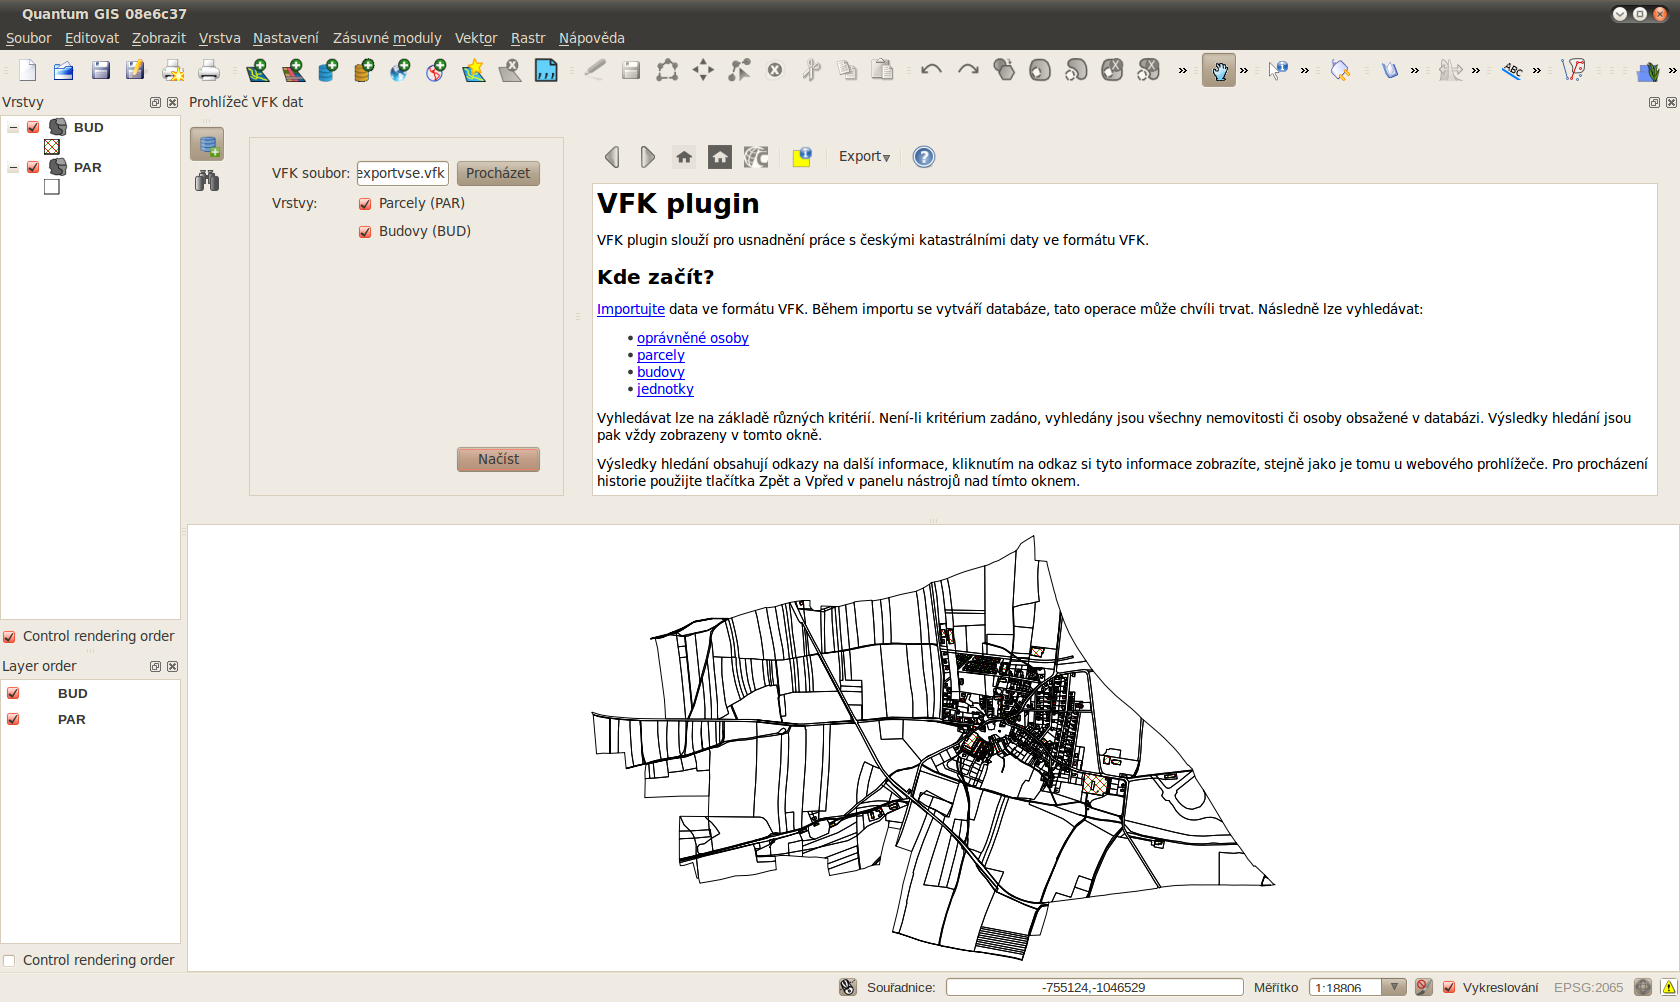
\includegraphics[width=\textwidth]{./screenshoty/Quantum_GIS_08e6c37_028.png}
% Quantum_GIS_08e6c37_028.png: 1680x1002 pixel, 72dpi, 59.27x35.35 cm, bb=0 0 1680 1002
\caption{QGIS se spuštěným VFK pluginem ukotveným v horní části.}
\label{fig:screenshot1}
\end{figure}

\begin{figure}[h!]
\centering
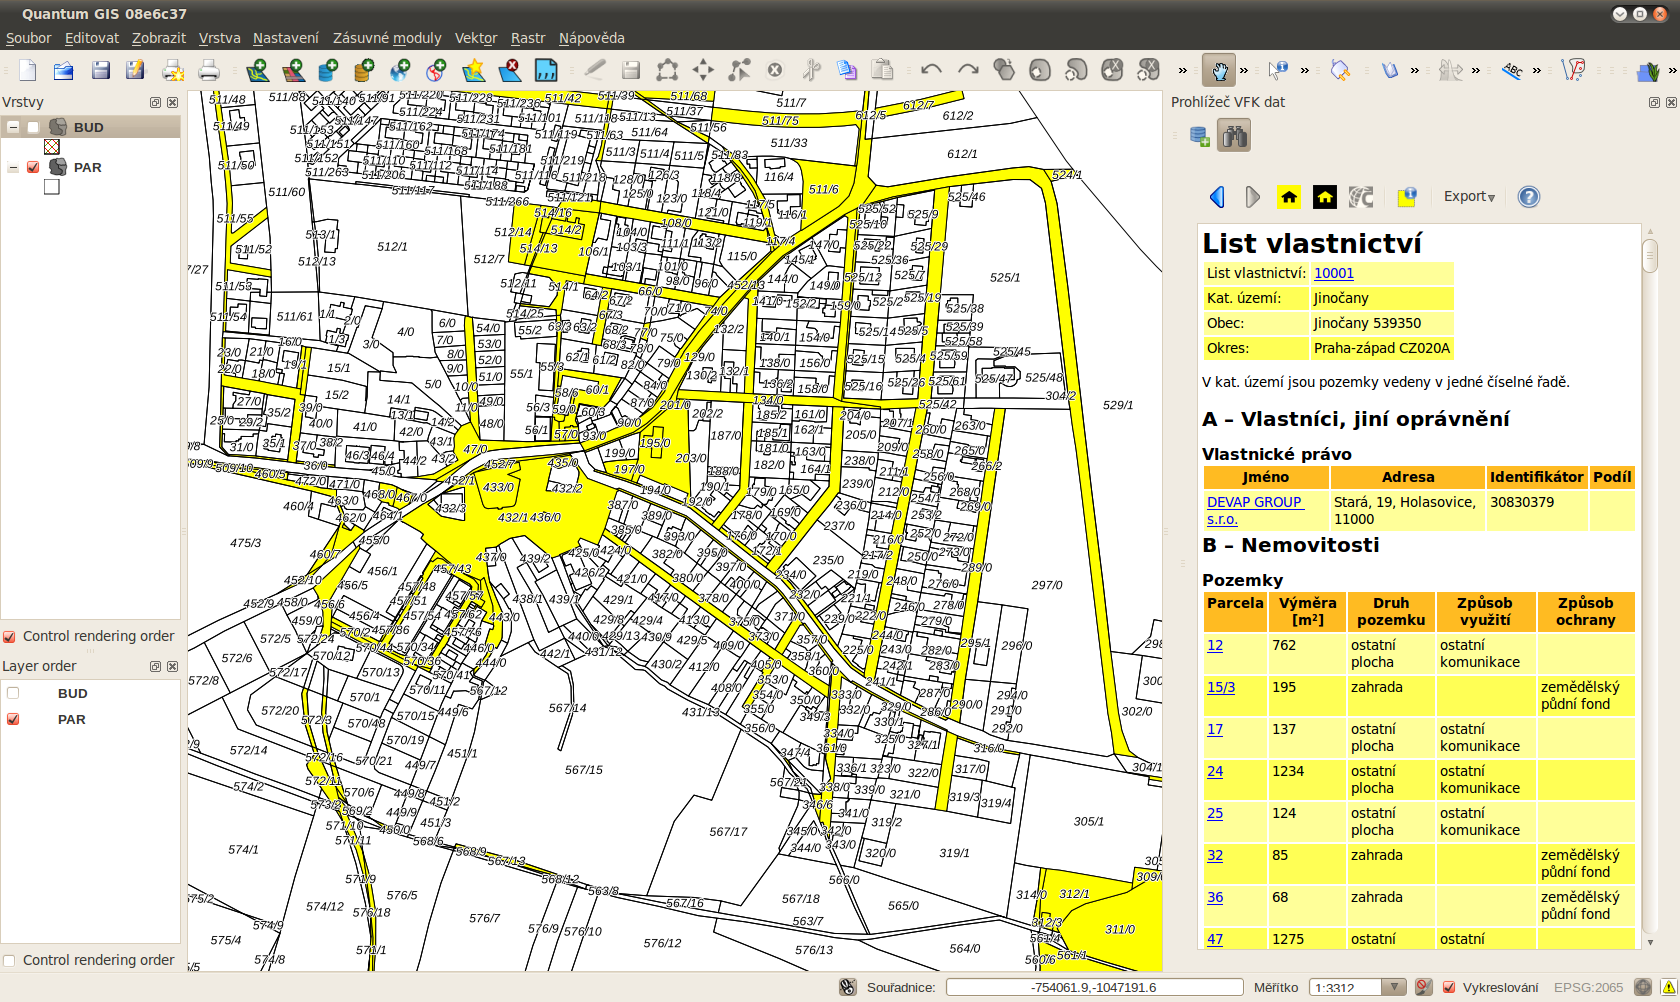
\includegraphics[width=\textwidth]{./screenshoty/Quantum_GIS_08e6c37_033.png}
% Quantum_GIS_08e6c37_028.png: 1680x1002 pixel, 72dpi, 59.27x35.35 cm, bb=0 0 1680 1002
\caption{Plugin v pravé části, v mapě jsou označeny nemovitosti na zobrazeném LV.}
\label{fig:screenshot2}
\end{figure}

\begin{figure}[h!]
\centering
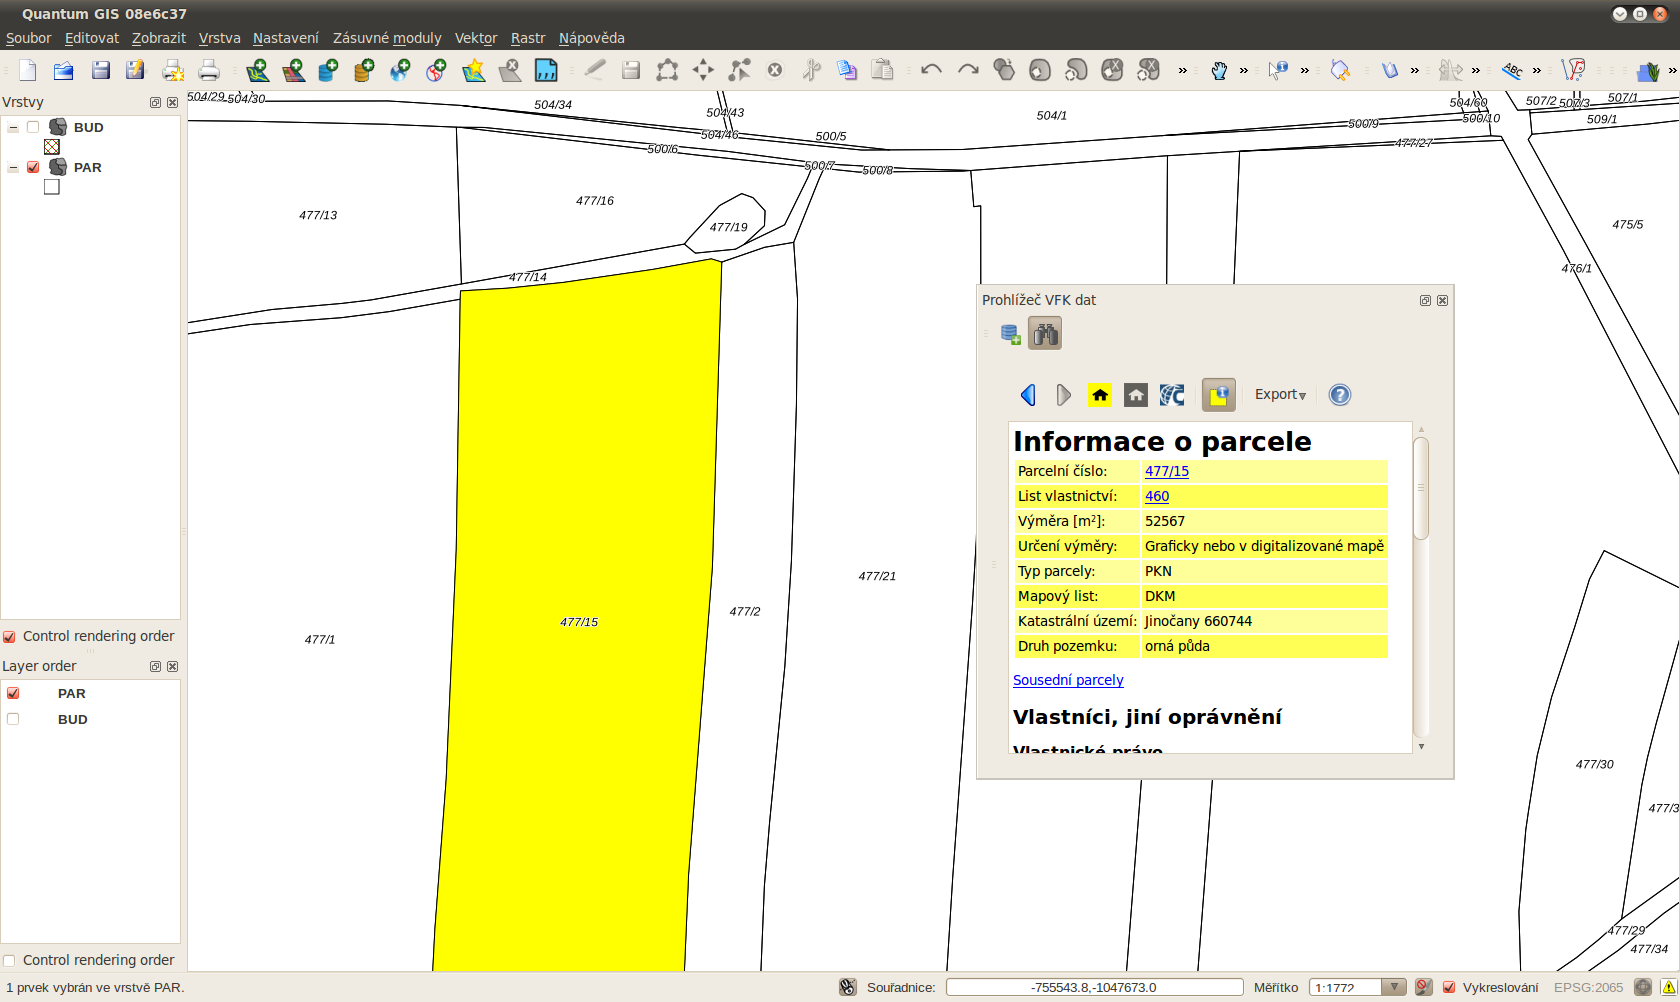
\includegraphics[width=\textwidth]{./screenshoty/Quantum_GIS_08e6c37_039.png}
% Quantum_GIS_08e6c37_028.png: 1680x1002 pixel, 72dpi, 59.27x35.35 cm, bb=0 0 1680 1002
\caption{Plugin stojící samostatně se skrytým ovládacím panelem.}
\label{fig:screenshot3}
\end{figure}
\clearpage
\section{Závěr}
Současná verze VFK pluginu implementuje základní funkcionalitu potřebnou pro prohlížení dat uložených ve výměnném formátu katastru (VFK).
Další funkcionalita se pude postupně přidávat především na základě ohlasů uživatelů.
V~tuto chvíli čeká plugin především testování.
Vzhledem k~tomu, že současná verze je jen prototyp, není plugin nijak oficiálně distribuován.
V~případě zájmu o~testování pluginu, či jinou spolupráci, neváhejte kontaktovat autory emailem:
    \begin{itemize}
    \item \verb|anna.kratochvilova fsv.cvut.cz|
    \item \verb|vaclav.petras fsv.cvut.cz|
    \end{itemize}
    
Prototyp VFK pluginu je poskytován zdarma pod licencí GNU GPL.

\newpage
\begin{tabular}{lp{10cm}}

\radekZkr{GNU}{GPL The GNU General Public License}
\radekZkr{GNU}{LGPL GNU Lesser General Public License}
\radekZkr{GPL}{viz GNU GPL}
\radekZkr{LGPL}{viz GNU LGPL}
\radekZkr{GNU}{GNU's Not Unix!; svobodný operační systém obvykle, a částečně chybně, označovaný jako Linux}

\radekZkr{SDK}{Software Development Kit, sada nástrojů pro vývoj softwaru}
\radekZkr{IDE}{Integrated Development Environment, vývojové prostředí}
\radekZkr{GUI}{Graphical User Interface}
\radekZkr{API}{Application Programming Interface}

\radekZkr{PDF}{Portable Document Format}
\radekZkr{ODF}{Open Document Format}
\radekZkr{XML}{Extensible Markup Language}
\radekZkr{HTML}{HyperText Markup Language}
\radekZkr{SQL}{Structured Query Language}

\radekZkr{GIS}{Geografický informační systém}

\radekZkr{VFK}{Výměnný formát katastru}
\radekZkr{NVF}{viz VFK, používáno při nutnosti rozlišit od starého výměnného formátu katastru}
\radekZkr{ISKN}{Informační systém katastru nemovitostí}

\radekZkr{GDAL}{Geospatial Data Abstraction Library}
\radekZkr{OGR}{OGR Simple Features Library}
\radekZkr{ESRI}{Environmental Systems Research Institute}
\radekZkr{QGIS}{Quantum GIS}

\end{tabular}

\begin{thebibliography}{9}

\bibitem{QtLicensing}
NOKIA. \textit{Qt Licensing, Frequently Asked Questions} [online]. [cit. 6. 4. 2012].
Dostupné z:~\textless\url{http://qt.nokia.com/about/licensing}\textgreater, \textless\url{http://qt.nokia.com/about/licensing/frequently-asked-questions}\textgreater.

\bibitem{QtLicensingDecision}
HAMLEY, Cristy. \textit{Qt: Making the right licensing decision} [online]. Qt Blog. 30. listopadu 2009, [cit. 6. 4. 2012]. Dostupné z: \textless\url{http://blog.qt.nokia.com/2009/11/30/qt-making-the-right-licensing-decision/} \textgreater.

\bibitem{vfkDriver}
GRASSwikiCZ. \textit{Výměnný formát ISKN} [online].
Naposledy editováno 8. 1. 2010, [cit. 10. 4. 2012]. Dostupné z: \textless
\url{
    http://grass.fsv.cvut.cz/wiki/index.php?title=V%C3%BDm%C4%9Bnn%C3%BD_form%C3%A1t_ISKN&oldid=2694
    } \textgreater

\bibitem{MartinThesis}
LANDA, Martin. \emph{Návrh modulu GRASSu pro import dat ve výměnném formátu ISKN} [online]. [cit. 2012-04-07]. Dostupné z: \textless\url{http://gama.fsv.cvut.cz/~landa/publications/2005/diploma_thesis/martin.landa-thesis.pdf}\textgreater. Diplomová práce. ČVUT Praha.

\bibitem{VFKDokumentace}
ČESKÝ ÚŘAD ZEMĚMĚŘICKÝ A~KATASTRÁLNÍ. \emph{Struktura výměnného formátu informačního systému katastru nemovitostí České republiky} [online]. 23. 2. 2012 [cit. 2012-04-07]. Dostupné z: \textless\url{http://www.cuzk.cz/GenerujSoubor.ashx?NAZEV=10-D12U}\textgreater.
    
    \end{thebibliography}
\end{document}
